\documentclass[a4paper,12pt,twoside]{apa}
\usepackage[left=2cm,right=2cm,top=2cm,bottom=3cm]{geometry}
\usepackage{apacite}
\usepackage{graphicx}
\usepackage{multirow}
\usepackage{tabularx}
\usepackage{float}
\usepackage{subcaption}
\usepackage{titling}
\usepackage[section]{placeins}

\title{\LARGE {\bf Extending WikiPathways to Improve Educational Capabilities}\\
 \vspace*{6mm}
}

\author{\textbf{Jacob Windsor} \\ \small{ORCID: 0000-0002-0249-7757}}

\begin{document}

\maketitle

{\raggedright{}
\textbf{Supervisor} \\
Egon Willighagen, \\
Department of Bioinformatics - BiGCaT, \\
Maastricht University, \\
Maastricht, \\
The Netherlands, \\
egon.willighagen@maastrichtuniversity.nl, \\
ORCID: 0000-0001-7542-0286

~\\
\textbf{Co-supervisor} \\
Anders Riutta, \\
The Gladstone Institutes,\\
San Francisco, \\
U.S.A, \\
anders.riutta@gladstone.ucsf.edu, \\
ORCID: 0000-0002-4693-0591

~\\
\textbf{Internal Supervisor} \\
FeiYian Yoong, \\
Maastricht Science Programme, \\
Maastricht University, \\
Maastricht, \\
The Netherlands, \\
feiyian.yoong@maastrichtuniversity.nl \\
}

\section{Background}
\subsection{Pathway Diagrams}
A pathway is a set of biological interactions between genes, proteins, or metabolites that drive a particular cellular function \cite{wu2010human}. Pathway diagrams are a useful abstraction to describe these biological processes. They enable simple visualisation of experimentally determined pathways \cite{bohler2016reactome}. Such diagrams have been used in biological research for many years and have helped biologists uncover the underlying mechanism for numerous phenomena such as respiration (Warburg), the tricarboxylic acid (TCA) cycle (Krebs), and the importance of ATP in energy transfer (Lipmann) \cite{deberardinis2012cellular}.

Pathway diagrams play an important role in understanding the progression of complex diseases, such as cancer, which occur as a result of an intricate interplay between metabolic, genetic and environmental factors. By using pathway diagrams in combination with ``omics'' data, the differences between biological interactions in normal cells and cancer cells can be elucidated. From this, possible targets for drug therapies can be determined. For example, metabolomic data has shown that cancer cells use macropinocytosis (the uptake of extracellular nutrients) to exploit extracellular proteins as an energy source for tumour growth \cite{commisso2013macropinocytosis}. Macropinocytosis has a role in normal cells but is over-stimulated in the presence of oncogenic RAS \cite{altman2016krebs}. Cancer cells use this increased activity to internalize extracellular proteins and degrade them into amino acids such as glutamine, a vital energy source for tumours \cite{commisso2013macropinocytosis, deberardinis2010q}. Hence, this metabolic pathway presents many targets for pharmacological inhibition (\textit{figure} \ref{pathway:cancer-cell-metabolism}}).

\begin{figure}[h]
  \centering
  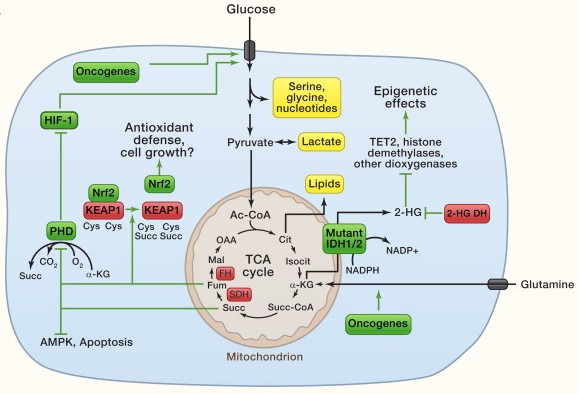
\includegraphics[scale=0.6]{figures/cancer-cell-metabolism.jpg}
  \caption{Cancer cell metabolism, showing the dependence on glutamine for metabolism. The uptake and catabolism of glucose and glutamine is regulated by tumour suppressors (red) and oncogenes (green). Metabolite pools fed by glutamine and glucose are highlighted in yellow. Oncogenes, tumour suppressors and metabolite pools are potential drug targets. \cite{deberardinis2012cellular}.}
  \label{pathway:cancer-cell-metabolism}
\end{figure}


\subsection{Dealing with an Abundance of Data}
Pathway diagrams are increasingly required to explain the complex biological networks that have arisen from the recent growth in biological data. High throughput ``omics'' technologies produce vast amounts of data that must be stored and understood \cite{bohler2016reactome}. Hence, many pathway databases have been created to store and facilitate the dissemination of this biological data. Currently, there are over 500 pathway databases in Pathguide, the pathway resource list, up from under 200 in 2005 \cite{bader2006pathguide, cary2005pathway}. The volume of pathways in these pathway databases makes them far more useful than pathway diagrams alone in the discovery of drug therapies for systemic diseases such as cancer and heart disease. These diseases are propagated by extensively interconnected pathways with high levels of redundancy \cite{ryall2015systems}. Thus, it is essential to understand the whole system of pathways leading to oncogenesis in order to find effective drug targets. Moreover, tumour cells are highly adaptive and can quickly develop resistance to any one drug by harnessing compensatory pathways \cite{dry2016looking}. Due to this, it is essential to develop drug combinations that target pathways that contribute to all aspects of tumour biology such as tumour cell metabolism, the tumour micro-environment, and immune response \cite{ryall2015systems}. In order to build an understanding of these complex networks of pathways, it is first essential to understand the mechanism of the component pathways individually. Pathway diagrams and databases are a significant aid in achieving this.

Despite the advantage of numerous pathway databases, researchers are finding it increasingly difficult to find and reuse data \cite{dumontier2016health}. Crucially, many databases do not provide pathway diagrams, with only 61 pathway diagram databases listed on Pathguide to date \cite{bader2006pathguide}. Furthermore, many databases demand expert knowledge to understand the pathways, meaning they are inaccessible to many scientists. This is in large part due to the fact that many pathways, such as in KEGG PATHWAY, are accompanied with insufficient or no descriptions to convey their role or mechanism of action \cite{kanehisa2004kegg}. Pathway curation is also a difficult task in many databases, requiring installation of complex software and specialized training. Thus, the barrier for both viewing and curating pathways is simply too high for many biologists. This leads to pathway curation and use being left to a small amount of specialists who have spent a significant amount of time developing a working knowledge of the available tools.

\subsection{WikiPathways - Pathways for the People}

WikiPathways aims to facilitate the contribution to and use of pathway information by the wider biological community. It is a community-driven, open-source, platform for curating and disseminating biological pathway knowledge, based upon the same wiki model as Wikipedia \cite{pico2008wikipathways}. It takes advantage of the wealth of knowledge in the scientific community by allowing anyone to create, edit, and view biological pathways rather than leveraging an internal curation team, such as in Reactome \cite{joshi2005reactome}. Furthermore, WikiPathways goes beyond conventional static pathway diagrams by utilising PathVisio, an interactive pathway diagram editor, to edit pathways, and a JavaScript version (PVJS) to view pathways (\textit{figure \ref{pathway:homo-sapiens-ovarian-cancer}}) \cite{kutmon2015pathvisio}. Significantly, this interactive editor enables easy curation of pathways by any biologist without extensive training. In addition, the integration of BridgeDb (a database identifier mapping framework) into the diagrams allows for easy access to gene, protein, and metabolite annotations \cite{van2010bridgedb, kelder2012wikipathways}. This interactivity drastically improves the educational capacity of pathway diagrams since readers can quickly find supplementary information. Additionally, pathways in WikiPathways are represented in the Graphical Pathway Markup Language (GPML), enhancing machine-readability and allowing use in downstream pathway analysis tools~\cite{kelder2012wikipathways}.

\begin{figure}[h]
  \centering
  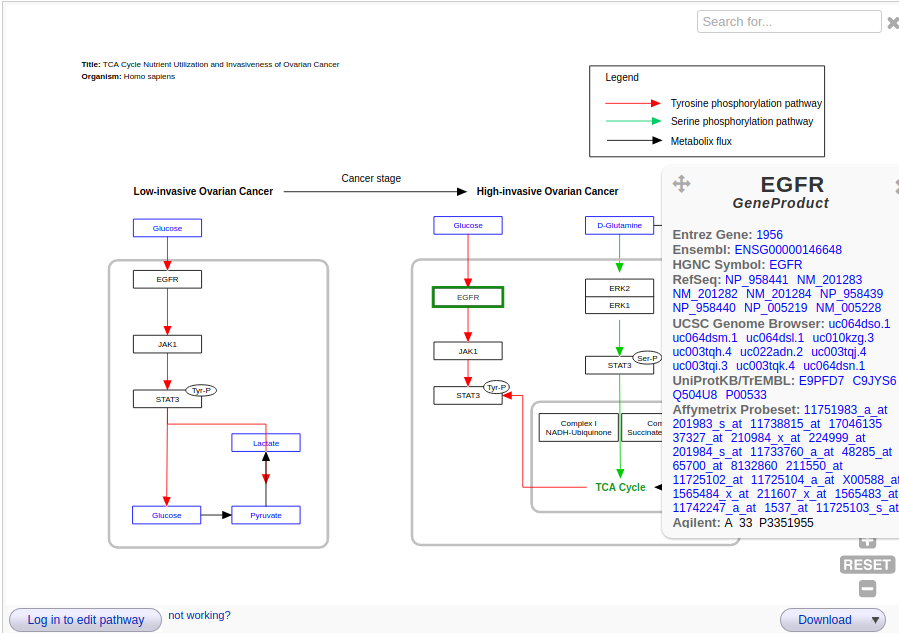
\includegraphics[scale=0.5]{figures/homo-sapiens-ovarian-cancer.png}
  \caption{TCA cycle nutrient utilisation and invasiveness of ovarian cancer in \textit{Homo sapiens} on WikiPathways. Dialogue box for the EGFR enzyme with various annotations shown.}
  \label{pathway:homo-sapiens-ovarian-cancer}
\end{figure}

\subsection{Limitations of WikiPathways}

Knowledge dissemination is improved in a multitude of ways in the wiki model over conventional scientific publishing \cite{hoffmann2008wiki}, but knowledge accessibility remains a  barrier to WikiPathways since it remains difficult for researchers to understand a pathway that outside their field. Thus, WikiPathways' educational capabilities must be improved to facilitate an intuitive and simple understanding of all pathways for the broad scientific community. One approach is to make the available descriptions interactive with hyperlinks that change the appearance of the diagram. This idea is successfully adopted by Proteopedia, a wiki for structural biology \cite{hodis2008proteopedia}. Proteopedia uses ``green hyperlinks'' within the text that change the three-dimensional visualisation of a biological molecule when clicked. In WikiPathways, the diagram could be altered to zoom in on the described interaction, highlight a particular region, or show annotations for a certain pathway element. Clicking a hyperlink would smoothly transition to a different pathway visualisation. These interactive descriptions will improve WikiPathways to convey pathway information in a more accessible manner, therefore, allowing researchers to build an understanding of biological processes from a field that they are not well versed in.

\section{Research Statement}
The educational capabilities of WikiPathways will be improved by the addition of interactive descriptions that manipulate the visualisation of the accompanying diagram.

\section{Proposed methods}
The interactive descriptions proposed here will first be tested in an educational cancer metabolism application before implementing them in WikiPathways. Two application flows to implement the interactive descriptions can be followed (\textit{Figure}~\ref{fig:cancer-app-both-flows}). These flows require initial changes to the application programming interfaces (APIs) of WikiPathways' component libraries, PVJS and Kaavio. The latter is a Javascript library used to render diagrams \cite{kaavio}, and the former is an abstraction on top of Kaavio to render WikiPathways specific pathways \cite{PVJS}. The choice of application flow is dependent on time constraints, with one being a fallback if the other fails to provide results in sufficient time. The methods for both flows are described herein.

A collaboration with Anders Riutta and others at the Gladstone Institutes will take place throughout the duration of this thesis.

\FloatBarrier
\subsection{Kaavio Manipulation API}
The preferred application flow utilises a ``manipulation API'' that provides Kaavio with methods to alter the diagram visualisation (\textit{figure \ref{fig:manipulation-api-flow}}). To this end, Kaavio will be extended with this API before usage in any application. The various methods, their parameters, and their functionalities are described in \textit{Table \ref{tbl:manipulation-api}}.

Although Kaavio is written in JavaScript, extensions will be written in Typescript, a typed superscript of JavaScript that compiles into regular JavaScript \cite{Typescript}. This supports debugging during development and ensures robust software.

Once complete, this API will allow developers to adapt the visualisation of pathways rendered in Kaavio.

\begin{table}[h]
\centering
\caption{Proposed manipulation API methods and their parameters.}
\label{tbl:manipulation-api}
\begin{tabularx}{0.9\textwidth}{|X|X|X|X|}
  \hline
  \multicolumn{2}{|C|}{\textbf{Method}} & \multicolumn{2}{|C|}{\textbf{Parameters}} \\ \hline
  \textbf{Name} & \textbf{Description} & \textbf{Name} & \textbf{Description} \\ \hline

  \multirow{2}{\hsize}{toggleHighlight} & \multirow{2}{\hsize}{Toggle highlighting of a target node (gene, metabolite, etc.)}
  & node\_id & The identifier of the target node. \\ \cline{3-4}
  & & colour & The desired colour to highlight with. \\ \hline

  resetHighlight & Reset all highlights. & - & - \\ \hline

  \multirow{2}{\hsize}{zoom} & \multirow{2}{\hsize}{Zoom in/out to a particular region.)}
  & zoom\_perc & The percentage to zoom (0-1). \\ \cline{3-4}
  & & origin & Object containing X and Y coordinates. \\ \hline

  zoomOn & Zoom into a particular node or group of nodes. & node\_id(s) & The identifier(s) of the target node(s). \\ \hline

  resetZoom & Reset zoom. & - & - \\ \hline

  pan & Pan to a coordinate. & coordinates & Object containing X and Y coordinates. \\ \hline

  panTo & Pan to a particular node or group of node. & node\_id(s) & The identifier(s) of the target node(s). \\ \hline

  resetPan & Reset pan to center. & - & - \\ \hline

  toggleAnnotations & Toggle the annotations for a particular node. & node\_id & The identifier of the target node. \\ \hline
\end{tabularx}
\end{table}

\FloatBarrier
\subsection{Direct Diagram Manipulation}
The development of the manipulation API within Kaavio may take a significant amount of time to complete. Thus, an alternative approach is proposed. Rather than altering Kaavio, the output pathway diagram from PVJS can be directly manipulated using cascading style sheets (CSS) (\textit{figure \ref{fig:direct-diagram-flow}}). This method only allows for the highlighting of data nodes and not other operations such as zooming and panning. If this approach is followed,  maintainability is significantly reduced since the single-responsibility principle is not followed \cite{martin2003agile}. Moreover, the difficulty of adding these new features to WikiPathways will be greatly increased.

\FloatBarrier
\subsection{Educational Cancer Metabolism Application}
In order to ensure the quality of the proposed additions, an educational cancer metabolism application will be developed. It will resemble WikiPathways and will detail different metabolic pathways and how they differ in oncogenic cells compared to normal cells. For example, the pathway for nutrient utilisation in the TCA cycle, as shown in \textit{Figure~\ref{pathway:homo-sapiens-ovarian-cancer}}, would be displayed alongside text describing the pathway and its differences in normal and cancer cells.  PVJS will be used to display the pathways. Additionally, accompanying pathway descriptions will contain interactive links that alter the displayed diagram.

The application will make use of multiple well-known application development tools to aid rapid development. Angular, a web application framework written in Typescript, will be used to structure and build the application logic~\cite{Angular}. Bootstrap, a popular user-interface framework, will be used to provide rapid prototyping for the application interface~\cite{Bootstrap}.

\begin{figure}[h]
  \centering
  \begin{subfigure}[b]{0.48\textwidth}
    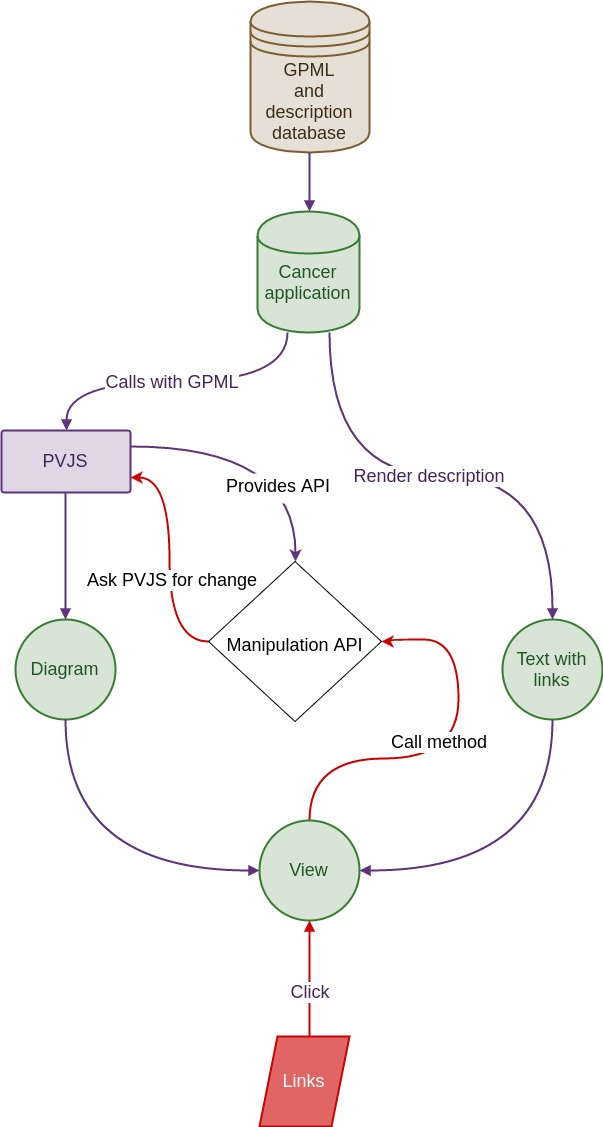
\includegraphics[width=\textwidth]{figures/manipulation_api.jpg}
    \caption{Application flow with Manipulation API. Upon clicking a link in the description, a manipulation API method is called which causes PVJS to alter the diagram visualisation.}
    \label{fig:manipulation-api-flow}
  \end{subfigure}
  \hspace*{\fill} % separation between the subfigures
  \begin{subfigure}[b]{0.48\textwidth}
    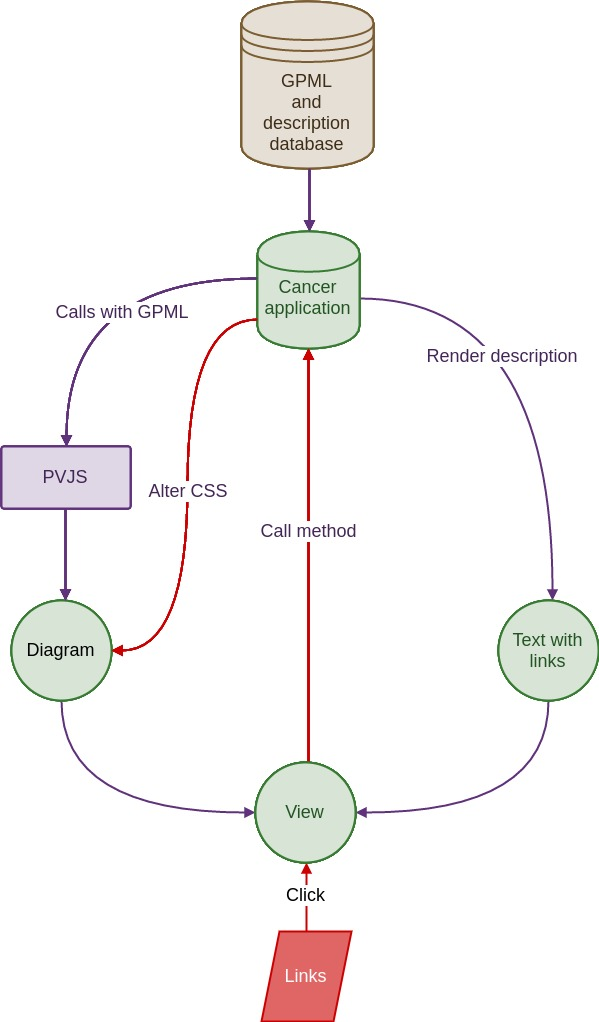
\includegraphics[width=\textwidth]{figures/direct.jpg}
    \caption{Application flow with direct diagram manipulation. Clicking a link in the description calls a method within the main application, which then alters the diagram's styling. PVJS has no knowledge of visualisation changes.}
    \label{fig:direct-diagram-flow}
  \end{subfigure}
  \caption{Flow diagrams for educational cancer metabolism application structures. Note that these flows can also be used in any application,  including WikiPathways.}
  \label{fig:cancer-app-both-flows}
\end{figure}

\FloatBarrier
\subsection{Testing}
The finished application will be tested amongst biomedical researchers and students but with varying degrees of experience in cancer metabolism. A set of questions, as outlined in \textit{Table \ref{tbl:test-questions}}, will be asked to determine the efficacy of the improvements. The testing will be an iterative process with feedback being taken into account, further improvements made if needed, and then further tested until satisfactory feedback is given. Once this process is complete, it can be concluded that the improvements are successful and ready to be used in WikiPathways itself.

\begin{table}[h]
  \centering
  \caption{Proposed questions for the cancer metabolism application testing. Two sets of questions will be given, before and after usage of the application.}
  \label{tbl:test-questions}
    \begin{tabularx}{0.9\textwidth}{|X|X|}
      \hline
      \textbf{Before use}
      &
      \textbf{After use}
      \\ \hline
      Do you have prior experience with WikiPathways? If so, for how long and what have you done (pathway creation, editing, viewing etc.)?
      &
      How easy was the application to use? In particular, did you find the interactive links within the description easily?
      \\ \hline
      Do you have any experience with other biological pathway databases? If so, which one(s)?
      &
      In general, do you think you have learnt about cancer metabolism via this application?
      \\ \hline
      Ranking from 0-10, how much knowledge do you have of cancer metabolism?
      &
      If you've used WikiPathways before, how much of an improvement are these interactive descriptions?
      \\ \hline
      &
      Do you have any further ideas for improvement?
      \\ \hline

    \end{tabularx}
\end{table}

\FloatBarrier
\subsection{Refactoring}
Aside from enabling interactive descriptions in WikiPathways, time will be spent on refactoring the existing PVJS codebase. Currently, PVJS is poorly structured with a weak distinction between Kaavio and PVJS. Thus, an attempt to rectify this will be carried out by re-writing PVJS and Kaavio in Typescript, using the React library for the user-interface~\cite{React, Typescript}. This will enhance the maintainability and allow for faster development because understandability will be increased. Note that refactoring will be done only if time allows.

\clearpage

\FloatBarrier
\subsection{Timeline}
The projected timeline for these methods is shown in \textit{table \ref{tbl:timeline}}.
\begin{table}[h]
  \centering
  \caption{Proposed timeline for the project. Dates approximate.}
  \label{tbl:timeline}
  \begin{tabularx}{0.9\textwidth}{|X|X|}
    \hline
    \textbf{Date} & \textbf{Goal} \\ \hline
    20th March & Assess if manipulation API can be completed and switch to direct diagram manipulation if not. \\ \hline
    17th April & Complete manipulation API or direct diagram manipulation. \\ \hline
    8th May & Complete educational cancer metabolism applicaton \& begin user testing. \\ \hline
    29th May & Finish user testing and perform any final improvements. \\ \hline
    Post-thesis & Add new improvements to WikiPathways \\ \hline
  \end{tabularx}
\end{table}

\section{Implications}

Biological pathway information is only valuable to the broad scientific community when it is part of a larger effort to communicate its role, mechanism, and implications. WikiPathways goes a great way to communicating pathways to the scientific community by integrating text-based descriptions and an interactive diagram~\cite{pico2008wikipathways}. The addition of interactive descriptions proposed here will increase the educational capabilities, allowing researchers to better understand and visualize their data. The potential consequences of this project reach beyond the WikiPathways and bioinformatics communities to the general biomedical research community. Interactive descriptions will aid information accessibility so that researchers can more easily understand a pathway from outside of their respective field. This is exemplified by Proteopedia, where the combination of descriptions and interactive 3D renderings of proteins aid communication complex information \cite{hodis2008proteopedia}. Ultimately, these improvements will support various biological fields, particularly in the understanding of complex, systemic biological phenomena such as cancer progression. By enabling researchers to interactively explore pathways, new insights into how best to manipulate them can be made.

\bibliographystyle{apacite}
\bibliography{references}

\end{document}
